\mychapter{Result and Discussion}
\vspace{0.5cm}

\subsection{Introduction}

This chapter walks through the experimental evaluation of the proposed \textbf{Digital Admission Script Evaluation and Moderation System (DASEMS)}. The goal here is to confirm that the implemented system actually meets its functional requirements and can carry the complete admission script evaluation workflow from start to finish. The evaluation looks at system functionality, document processing, the evaluation workflow itself, and how well everything holds together as an integrated whole.

\subsection{Experimental Setup}

The system was tested using a prototype admission examination setup built from a React frontend, a Node.js backend, a MongoDB database, and a Python-based document processing service. The experiments ran on scanned admission answer scripts covering Physics, Chemistry, Mathematics, and English.

All three user roles -- \textbf{Super Administrator}, \textbf{Head Examiner}, and \textbf{Teacher} -- were exercised to validate the full workflow, from PDF processing and question segmentation through teacher assignment, evaluation, moderation, and result generation.

\begin{table}[H]
\centering
\caption{Experimental Environment}
\label{tab:experimental_environment}
\renewcommand{\arraystretch}{1.2}

\begin{tabular}{|p{5cm}|p{7.5cm}|}
\hline
\textbf{Component} & \textbf{Configuration} \\
\hline
Frontend & React 18 (TypeScript) \\
\hline
Backend & Node.js with Express.js \\
\hline
Database & MongoDB \\
\hline
Document Processing & Python FastAPI \\
\hline
PDF Library & PyMuPDF \\
\hline
OCR Engine & Tesseract OCR \\
\hline
Authentication & JWT, bcrypt \\
\hline
Deployment & Docker Compose \\
\hline
Operating System & macOS \\
\hline
Dataset & Sample Admission Answer Scripts \\
\hline
Subjects & Physics, Chemistry, Mathematics, English \\
\hline
User Roles & Super Administrator, Head Examiner, Teacher \\
\hline
\end{tabular}

\end{table}

\subsection{Functional Evaluation}

Functional evaluation checked that every module worked correctly on its own and that the full admission evaluation workflow ran successfully once everything was connected. Modules were tested individually first, then validated again as part of the integrated system.

This covered user authentication, admission management, PDF processing, question segmentation, teacher assignment, evaluation, moderation, and result generation. Table~\ref{tab:functional_evaluation} summarizes what came out of this testing.

\begin{table}[H]
\centering
\caption{Functional Evaluation Results}
\label{tab:functional_evaluation}
\renewcommand{\arraystretch}{1.2}

\begin{tabular}{|p{6cm}|p{6cm}|p{1.6cm}|}
\hline
\textbf{Module} & \textbf{Expected Outcome} & \textbf{Status} \\
\hline
Authentication & Secure user login & Pass \\
\hline
Admission Management & Session and student management & Pass \\
\hline
PDF Processing & Question regions extracted & Pass \\
\hline
Teacher Assignment & Automatic task allocation & Pass \\
\hline
Evaluation & Marks submitted successfully & Pass \\
\hline
Moderation & Conflicting evaluations resolved & Pass \\
\hline
Result Generation & Final results generated & Pass \\
\hline
Audit Logging & User activities recorded & Pass \\
\hline
\end{tabular}

\end{table}

Every module tested here worked as expected, and the full workflow ran end to end without any critical failures.

\subsection{Workflow Validation}

Beyond testing modules on their own, the complete workflow was run through as an integrated platform to make sure everything worked together properly.

The process started with the Super Administrator setting up an admission session, uploading the question bank, registering students, and submitting scanned answer scripts. The backend checked each uploaded document and passed the valid ones along to the Python document processing service, which handled rendering, hybrid question detection, answer extraction, and metadata generation.

Once extracted, answer records went into MongoDB and were automatically routed to subject-specialized teachers based on the workload-balancing rules already in place. Teachers then worked through their assigned answers in the browser, using the digital annotation tools to mark up scripts and submit their marks.

After all three independent evaluations for an answer came in, the moderation module compared the marks. Anything that crossed the moderation threshold went to the Head Examiner; everything else was finalized automatically. From there, the result generation module worked out student scores and put together the examination reports.

\begin{table}[H]
\centering
\caption{Workflow Validation Results}
\label{tab:workflow_validation}
\begin{tabular}{|p{6cm}|p{5cm}|p{2cm}|}
\hline
\textbf{Workflow Stage} & \textbf{Validation Outcome} & \textbf{Status} \\
\hline
User Authentication & Authorized access verified & Pass \\
\hline
Admission Configuration & Session created successfully & Pass \\
\hline
PDF Upload and Validation & Documents processed correctly & Pass \\
\hline
Question Detection & Questions identified successfully & Pass \\
\hline
Answer Extraction & Answer regions extracted & Pass \\
\hline
Teacher Assignment & Automatic allocation completed & Pass \\
\hline
Evaluation Submission & Marks stored successfully & Pass \\
\hline
Moderation Workflow & Threshold-based moderation executed & Pass \\
\hline
Result Generation & Final results generated correctly & Pass \\
\hline
\end{tabular}
\end{table}

\begin{figure}[H]
    \centering
    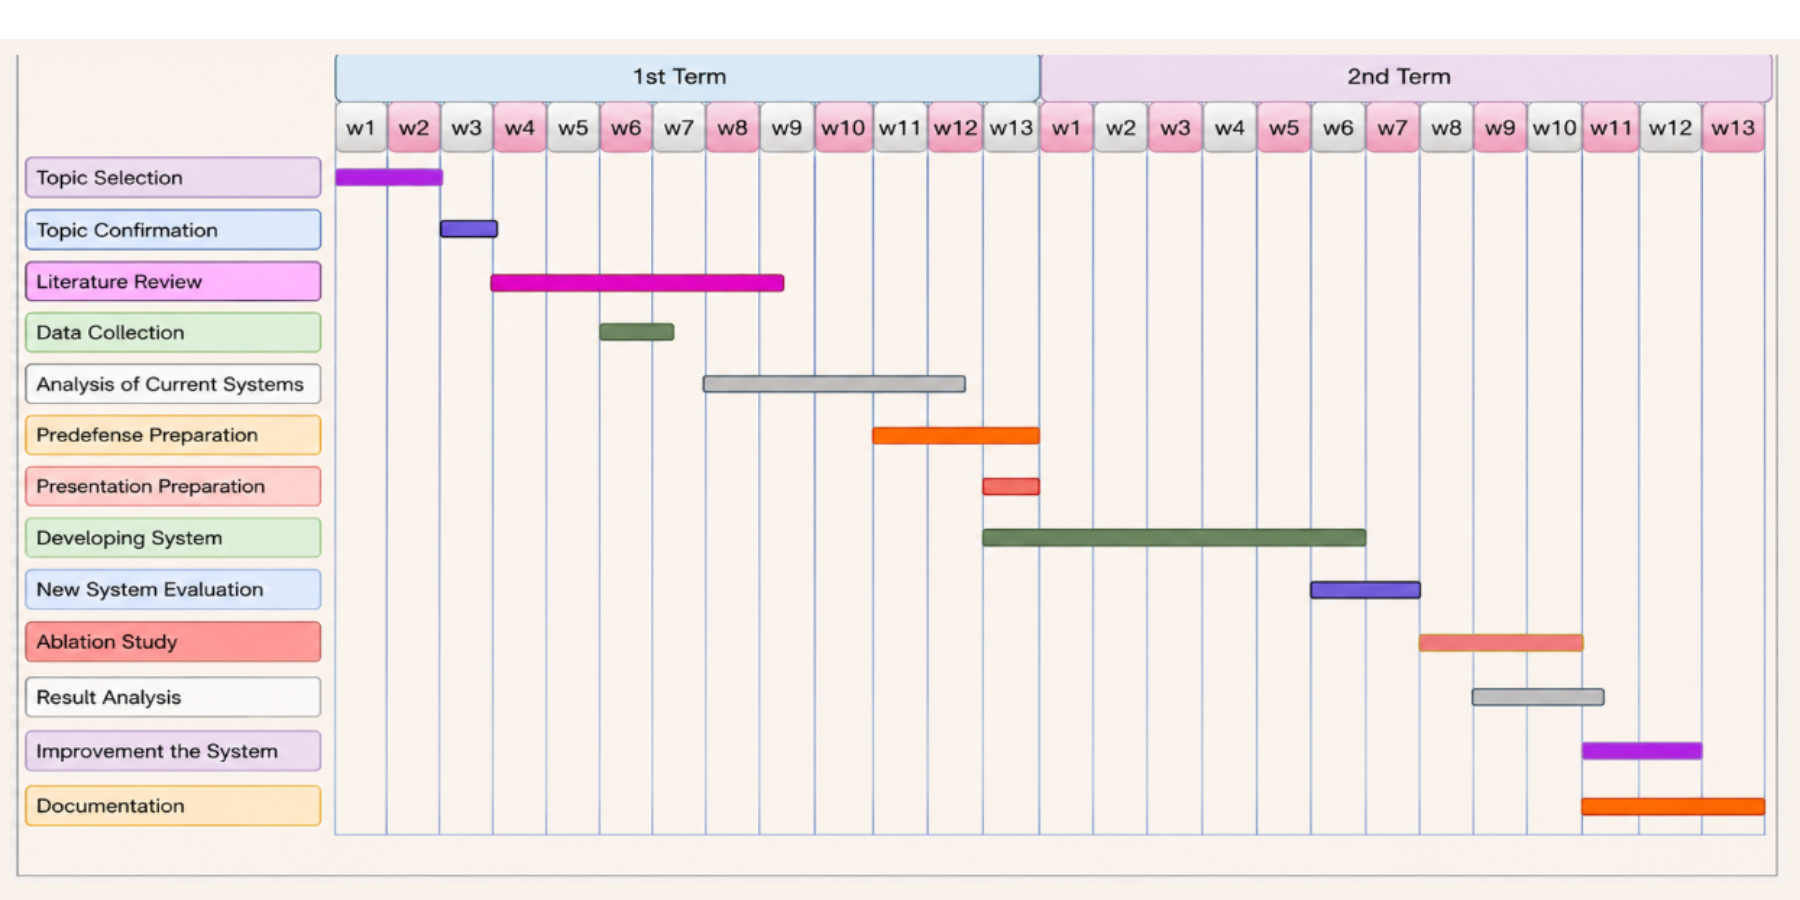
\includegraphics[width=1.0\textwidth]{img/workflow.png}
    \caption{Entire Project Workflow.}
    \label{fig:Entire Project Workflow}
\end{figure}

\subsection{Performance Analysis}

Performance testing looked at how responsive DASEMS is and how efficiently it moves through the evaluation workflow during a descriptive admission examination.

Because the architecture keeps the React frontend, Node.js backend, MongoDB database, and Python document processing service as separate pieces, the heavier work -- PDF processing and OCR -- runs on the Python service without dragging down the responsiveness of the web application itself.

The React frontend only re-renders what actually changes, and indexed MongoDB collections keep data retrieval fast. PDF processing and answer extraction both run asynchronously, so administrators and teachers can keep working while documents are being processed in the background.

The evaluation interface only pulls in answers that are actually assigned to a given teacher, which cuts down on unnecessary data loading, and the automated assignment and moderation modules let evaluation happen in parallel while keeping administrative overhead low.

\begin{table}[H]
\centering
\caption{Performance Analysis Summary}
\label{tab:performance_analysis}
\begin{tabular}{|p{6cm}|p{5cm}|p{2cm}|}
\hline
\textbf{Performance Aspect} & \textbf{Observation} & \textbf{Status} \\
\hline
Frontend Responsiveness & Smooth navigation and UI updates & Good \\
\hline
Backend API Response & Stable communication with frontend & Good \\
\hline
Database Operations & Fast retrieval using indexes & Good \\
\hline
PDF Processing & Executed asynchronously & Good \\
\hline
Teacher Assignment & Balanced workload distribution & Good \\
\hline
Evaluation Workflow & Parallel evaluation supported & Good \\
\hline
Moderation Process & Triggered only when required & Good \\
\hline
Overall System Integration & Stable during end-to-end workflow & Good \\
\hline
\end{tabular}
\end{table}
\FloatBarrier

Taken together, these observations suggest the system holds up well under the demands of a descriptive admission examination -- responsive and reliable throughout. The modular architecture, asynchronous PDF processing, efficient database design, and automated workflow all point toward a system that could scale to larger evaluations and eventually move to a cloud deployment.

\subsection{Discussion}

The results here show that DASEMS meets the objectives laid out back in Chapter I. Bringing together document processing, secure web technologies, and automated workflow management gives this system a real, practical answer to the problems universities run into when evaluating descriptive admission exams.

One of the bigger wins here is how much administrative work gets automated before evaluation even starts. The PDF processing module pulls question-wise answer images out of uploaded scripts on its own, so nobody has to manually separate questions, which saves a meaningful amount of prep time. The hybrid strategy -- pulling embedded PDF text where it exists, falling back to OCR where it doesn't -- keeps things efficient while still handling both searchable and scanned PDFs.

Keeping student identities hidden from teachers throughout evaluation makes the process fairer by design. On top of that, automated teacher assignment spreads answers out by subject specialization and workload, letting evaluation run in parallel while making sure no evaluator can see what the others scored.

Moderation adds another layer of reliability, but a targeted one -- only disputed evaluations actually reach the Head Examiner, so moderation doesn't become a bottleneck while consistency and transparency stay intact. The modular split between frontend, backend, document processing, and database also means the system is easier to maintain and has room to grow.

That said, the system isn't without its limits. The document processing module works from the assumption that exam layouts stay fairly consistent, so a script with a very different template would need extra configuration to handle. And to be clear, this system doesn't grade handwritten answers itself -- the actual academic judgment stays entirely with human examiners.

It's also worth noting that this prototype was tested in a controlled setting, using a representative but limited set of admission scripts. The results here point to the approach being workable, but rolling it out at full institutional scale would say a lot more about how it holds up over time and under heavier load.

Even with those caveats, DASEMS offers a clear step up from paper-based evaluation -- automated document processing, anonymous grading, centralized moderation, and automated results, all in one platform. And because of how it's built, there's a solid foundation here for adding things later, like AI-assisted handwriting recognition, smarter answer analysis, or a full cloud deployment.

\subsection{Chapter Summary}

This chapter covered the experimental evaluation of DASEMS -- functional testing, workflow validation, performance analysis, and a discussion of what it all means. Across the board, the evaluation confirmed that the system meets the objectives set out for this research.

Every major module -- authentication, PDF processing, question detection, answer extraction, teacher assignment, evaluation, moderation, and result generation -- worked correctly within the integrated system.

On the performance side, the modular architecture, asynchronous document processing, and optimized database operations kept the system responsive throughout the evaluation process, while automated teacher assignment and digital result generation added further gains in efficiency and transparency for descriptive admission examinations.

All told, DASEMS offers a practical, secure digital platform that cuts down manual administrative work considerably while making descriptive university admission examinations fairer and more efficient to run.

The next chapter closes out the thesis, summarizing the research contributions, discussing where the system falls short, and laying out directions for future work.